%%%%%%%%%%%%
% Preamble %
%%%%%%%%%%%%
\input{../preamble.tex}
\title{Axiomatic Set Theory}
\author{Aiken Ji}
\date{\today}

%%%%%%%%%%%%
% Document %
%%%%%%%%%%%%

\begin{document}
\maketitle

\newpage

\definecolor{tcol_CNT1}{HTML}{72E094} % First color for Contents
\definecolor{tcol_CNT2}{HTML}{24E2D6} % Second color for Contents
\definecolor{tcol_CNV1}{HTML}{8E44AD} % First color for Conventions
\definecolor{tcol_CNV2}{HTML}{A10B49} % First color for Conventions

\begin{tcolorbox}[enhanced,
    title=Contents,
    fonttitle=\fontsize{20}{24}\sffamily\bfseries\selectfont,
    coltitle=black,
    fontupper=\sffamily,
    interior style={left color=tcol_CNT1!80,right color=tcol_CNT2!80},
    frame style={left color=tcol_CNT1!60!black,right color=tcol_CNT2!60!black},
    attach boxed title to top center={yshift=10pt},
    boxed title style={frame hidden,
      interior style={left color=tcol_CNT1,right color=tcol_CNT2},
      frame style={left color=tcol_CNT1!60!black,right
      color=tcol_CNT2!60!black},
      height=24pt,bean arc,drop fuzzy shadow
    },
    top=2mm,bottom=2mm,left=2mm,right=2mm,
    before skip=20mm,after skip=20mm,
  drop fuzzy shadow,breakable]
  %
  \makeatletter
  \@starttoc{toc}
  \makeatother
\end{tcolorbox}

\begin{tcolorbox}[enhanced,
    frame hidden,
    title=Conventions,
    fonttitle=\large\sffamily\bfseries\selectfont,
    interior code={
      \shade[top color=tcol_CNV2!50,bottom color=white]
      ([yshift=2mm]interior.north west)
      arc(-180:-90:2mm)--(interior.north east)--(interior.south
      east)--(interior.south west)--cycle;
    },
    overlay={
      \draw[tcol_CNV1!50!black,line width=0.5mm]
      ([xshift=2mm]frame.north west)--(frame.north east);
    },
    boxrule=0pt,left=2pt,right=2pt,
    sharp corners=north,
    attach boxed title to top left,
    boxed title style={interior hidden,
      left=1mm,right=1mm,
      frame code={
        \path[draw=tcol_CNV1!50!black,line
        width=0.5mm,fill=tcol_CNV1,rounded corners=2mm]
        ([xshift=2mm]frame.south east)--(frame.south
        east)--(frame.north east)--([xshift=0.25mm]frame.north
      west)--([xshift=0.25mm]frame.south west)--cycle;}
    },
    top=2mm,bottom=2mm,left=2mm,right=2mm,
  before skip=10mm,after skip=10mm]
  %
  $\F$ denotes either $\R$ or $\C$.\\
  $\N$ denotes the set $\{1,2,3,\ldots\}$ of natural numbers (excluding $0$).\\
  Inner products are taken to be linear in the first argument and
  conjugate linear in the second.\\
  The Einstein summation convention is used for tensors unless
  otherwise specified.
\end{tcolorbox}

\newpage

\section{Language of set theory}

\subsection{Basic Set-Building Axioms}

We construct a formal language suitable for describing sets. The
language consists of some mathematical symbols as well as purely
logical symbols.

The complete list of symbols of language is as below:
\begin{definition}{Symbols in LOST(Language of Set Theory)}{}
    \begin{enumerate}
        \item variable: $v_0, v_1, v_2, \ldots$
        \item equality: $=$
        \item membership: $\in$
        \item connectives: $\neg, \land, \lor, \implies, \iff$
        \item quantifiers: $\forall, \exists$
        \item parentheses: $\left(,\ \right)$
    \end{enumerate}
\end{definition}

\begin{remarks}
    Bounded set quantifiers shall be used. You can abbreviate the formula:
    \begin{enumerate}
        \item $\forall x (x \in y \implies x \notin a)$ by $(\forall x
            \in y) (x \notin a).$
        \item $\exists x (x \in y \land x \notin a)$ by $(\exists x \in
            y) (x \notin a).$
    \end{enumerate}
\end{remarks}

\begin{definition}{Zermelo-Fraenkel Axioms}{}
    \begin{enumerate}
        \item \textbf{Extensionality Axiom.}\\
            Two sets are equal iff they have the same elements.\\
            \\
            $\forall A \forall B (A=B \iff \forall x (x \in A \iff x \in B))$ \\
        \item \textbf{Empty Set Axiom.} \\
            There is a set with no elements.\\
            \\
            $\exists A \forall x (x \notin A)$\\
        \item \textbf{Subset Axiom.} \\
            Let $\varphi(x)$ be a formula. For every set $A$ there exists a
            set $S$ that consists of all $x \in A$ with $\varphi(x)$ holds.\\
            \\
            $\forall A \exists S \forall x (x \in S \iff (x \in A \wedge
            \varphi(x))) $\\
        \item \textbf{Pairing Axiom.}\\
            For every $u$ and $v$ there is a set that consists of
            just $u$ and $v$.\\
            \\
            $\forall u \forall v \exists S \forall x (x \in S \iff (x = u
            \vee x = v)) $\\

        \item \textbf{Union Axiom.}\\
            For every set $\mathcal{F}$ there exists a set $U$ that
            consists of all elements that belong to at least one set in
            $\mathcal{F}$.\\
            \\
            $\forall \mathcal{F} \exists U \forall x (x \in U \iff \exists
            F \in \mathcal{F} (x \in F))$\\
        \item \textbf{Power Set Axiom.}\\
            For every set $A$ there is a set $\mathcal{P}$ that consists of
            all subsets of $A$.\\
            \\
            $\forall A \exists \mathcal{P} \forall P (P \in \mathcal{P}
            \iff P \subseteq A)$
    \end{enumerate}
\end{definition}

\begin{remarks}
    \begin{enumerate}
        \item The empty set axiom defines the \textbf{empty set} denoted
            by $\varnothing$.
        \item The subset axiom defines the set denoted by $\{x \in
            A:\varphi(x)\}$.
        \item The pairing axiom defines the \textbf{unordered pair}
            denoted by $\{u, v\}$. If $u = v$, then the set
            $\left\{u\right\}$ is referred to as a \textbf{singleton}.
        \item The union axiom defines the \textbf{union} of $\mathcal{F}$
            denoted by $\bigcup \mathcal{F}$.
        \item The power set axiom defines the \textbf{power set} of $A$
            denoted by $\mathcal{P}(A) = \{X:X \subseteq A\}.$
    \end{enumerate}
\end{remarks}

\begin{definition}{Class}{}
    We shall refer to any collection of the form $\{x:\varphi(x)\}$ as
    a \textbf{class}. We call it \textbf{proper class},
    when the class is not a set, such as $\{x:x=x\}$. Sometimes we also
    call it \textbf{unbounded collection.}
\end{definition}

\begin{theorem}{Sufficient condition for class to be a set}{label:class}
    Let $\varphi(x)$ be a formula. Suppose that there is a set $A$ such
    that for every $x$, if $\varphi(x)$, then $x \in A$. Then there is
    a unique set $S$ such that for all $x$, $x \in S \iff \varphi(x)$.\\
    \begin{equation*}
        \exists A \forall x (\varphi(x) \implies x \in A) \implies
        \exists ! S \forall x(x \in S \iff \varphi(x))
    \end{equation*}
    \\
    In other words, the class $\{x:\varphi(x)\}$ is equal to the set $S$.
\end{theorem}

\begin{proof}
    Let $S = \left\{x \in A \colon \varphi(x) \right\}$ which is
    uniquely defined by subset axiom.\\
    ($ \implies $)\\
    $x \in S \implies x \in A \land \varphi(x) \implies \varphi(x).$\\
    ($ \Leftarrow $)\\
    $\varphi(x) \implies x \in A \implies x \in A \land \varphi(x)
    \implies x \in S.$
\end{proof}
\begin{remarks}
    Furthermore, the sufficient and necessary condition for class to be
    a set is as follows:
    \begin{equation*}
        \exists S \forall x(x \in S \iff \varphi(x)) \iff \exists A
        \forall x(\varphi(x) \implies x \in A)
    \end{equation*}
\end{remarks}

\begin{corollary}{}{}
    Let $\varphi(x)$ be a formula. Then $\{x:\varphi(x)\}$ is a proper
    class iff for every set $A$ there is a $x$ s.t. $\varphi(x)$ and
    $x \notin A$.

\end{corollary}
By the \Cref{class}, Some sets operations below are well defined and
can be used to create new sets.

\begin{corollary}{}{}
    Union, Intersection and Difference of sets can be defined by
    \Cref{class}. For any set $A$, $B$ and nonempty collection $\mathcal{F}$:\\
    \begin{enumerate}
        \item Union: $A \cup B = \{x: x \in A \lor x \in B\} $
        \item Intersection: $A \cap B = \{x: x \in A \land x \in B\}$
        \item Difference: $A \setminus B = \{x: x \in A \land x \notin B\}$
        \item Union of $\mathcal{F}$: $\bigcup \mathcal{F} = \{x: \exists
            F \in \mathcal{F}(x\in F)\}$
        \item Intersection of $\mathcal{F}$: $\bigcap \mathcal{F} = \{x:
            \forall F \in \mathcal{F}(x\in F)\}$
    \end{enumerate}
\end{corollary}

\begin{remark}
    If collection $\mathcal{F}$ is empty, then\\
    \begin{enumerate}
        \item $\bigcup \varnothing = \varnothing$
        \item $\bigcap \varnothing$ is not well defined as set. Because
            the statement $x$ belongs to every members of empty set is
            vacuously true. So all x will belongs to it, which is a
            contradiction.
    \end{enumerate}
\end{remark}

\begin{theorem}{}{}
    Suppose nonempty sets $\mathcal{F}$, $\mathcal{G}$ and $\mathcal{F}
    \subseteq \mathcal{G}$. Then $\bigcup \mathcal{F} \subseteq \bigcup
    \mathcal{G}$ and $\bigcap \mathcal{G} \subseteq \bigcap \mathcal{F}$.
\end{theorem}

\begin{proof}
    To proof the first one, Let $x \in \bigcup \mathcal{F}$.
    \begin{align*}
        &\implies x \in F \ \text{for some}\ F \in \mathcal{F} \land
        \mathcal{F} \subseteq \mathcal{G} \\
        &\implies x \in F \ \text{for some}\ F \in \mathcal{G}\\
        &\implies x \in \bigcup \mathcal{G}\\
        &\implies \bigcup \mathcal{F} \subseteq \bigcup \mathcal{G}\\
    \end{align*}
\end{proof}

\newpage

\subsection{Operations on Sets}

There are some other important ways to build new sets by axioms in
previous section.

\begin{lemma}{}{}
    Let $A$ and $\mathcal{F}$ be sets. Then there is a unique set
    $\mathcal{C}$ such that for all $X$,
    \begin{equation*}
        X \in \mathcal{C} \iff X = A \setminus F\ \text{for some}\ F
        \in \mathcal{F}
    \end{equation*}
    or,
    \begin{equation*}
        X \in \mathcal{C} \iff \exists F \in \mathcal{F}(X = A \setminus F)
    \end{equation*}
    We shall denote $\mathcal{C}$ by $\{A \setminus F: F \in \mathcal{F}\}$.
\end{lemma}

\begin{proof}
    $\exists F \in \mathcal{F}(X = A \setminus F) \implies X \subseteq
    A \implies X \in \mathcal{P}(A)$\\
    by \Cref{class}, set $\mathcal{C}$ is uniquely constructed.

\end{proof}

\begin{theorem}{De Morgan's Laws}{DML}
    If $A$ is a set and $\mathcal{F}$, then
    \begin{eqnarray*}
        A \setminus \bigcup \mathcal{F} = \bigcap \{A \setminus F: F \in
        \mathcal{F}\}\\
        A \setminus \bigcap \mathcal{F} = \bigcup \{A \setminus F: F \in
        \mathcal{F}\}
    \end{eqnarray*}
\end{theorem}

\begin{proof}
    Proof the first one.\\
    \begin{align*}
        x \in A \setminus \bigcup \mathcal{F} &\iff x \in A \land x
        \notin \bigcup \mathcal{F}\\
        &\iff x \in A \land (\forall F \in \mathcal{F}(x \notin F)) \\
        &\iff \forall F \in \mathcal{F}(x \in A \land x \notin F)\\
        &\iff \forall F \in \mathcal{F}(x \in A \setminus F)\\
        &\iff x \in \bigcap \{A \setminus F : F \in \mathcal{F}\}
    \end{align*}
\end{proof}

\newpage
\section{Relations and Functions}
\subsection{Ordered Pairs}
In mathematics, relations and functions are usually defined in terms
of ordered pairs. The key property the ordered pairs satisfied is as below
\begin{definition}{Ordered Pairs}{}
    Basic property the ordered pairs should satisfy, which is also the
    axiomatic definition of ordered pairs
    \begin{equation*}
        \langle a,b \rangle = \langle c,d \rangle \iff a = b \land c = d
    \end{equation*}
\end{definition}
In 1921, Kazimierz Kuratowski give the construction of ordered pair
based on ZF systems.
\begin{definition}{Set Based Construction of Ordered Pairs}{}
    The \textbf{ordered pair}, with first component x and second
    component y, is the set defined by
    \begin{equation*}
        \langle x,y \rangle = \{\{x\}, \{x, y\}\}
    \end{equation*}
\end{definition}

\begin{lemma}{}{}
    Let $A$, $B$ be sets, there exists a unique set $\mathcal{D}$ s.t.
    for all $X$,
    \begin{equation*}
        X \in \mathcal{D} \iff X = \langle x,y \rangle \ \text{for
        some}\ x \in A \land y \in B.
    \end{equation*}
    or,
    \begin{equation*}
        X \in \mathcal{D} \iff (\exists x \in A)(\exists y \in B)(X =
        \langle x,y \rangle)
    \end{equation*}
    We shall denote $\mathcal{D}$ by $\{\langle x,y \rangle : x \in A
    \land y \in B\}$.
\end{lemma}

\begin{proof}
    $X = \langle x,y \rangle \ \text{for some}\ x \in A \land y \in B
    \implies X = \{\{x\},\{x,y\}\} \in \mathcal{P}(\mathcal{P}(A \cup B) )$.\\
    The set $\mathcal{D}$ is uniquely defined by \Cref{class}.
\end{proof}

\begin{definition}{Cartesian Product}{}
    Given sets $A$ and $B$, the \textbf{Cartesian product} $A \times B$
    is defined to be the set
    \begin{equation*}
        A \times B = \{\langle x,y \rangle : x \in A \land y \in B\}
    \end{equation*}
    which is uniquely given by the above lemma.
\end{definition}

\subsection{Relations}
\begin{definition}{Relations}{}
    A \textbf{Relation} $R$ is a set of orded pairs. In other words,
    for all $x$,
    \begin{equation*}
        x \in R \iff x = \langle a,b \rangle \ \text{for
        some}\ a\ \text{and}\ b.
    \end{equation*}
\end{definition}

\begin{definition}{}{}
    Let $A$ and $B$ be sets.
    \begin{enumerate}
        \item A \textbf{relation from $A$ to $B$} is a subset of $A
            \times B$, or $R \subseteq A \times B$.
        \item A \textbf{relation on $A$} is a subset of $A \times A$, or
            $R \subseteq A \times A$.
    \end{enumerate}
\end{definition}

\begin{remarks}
    by subset axiom, given a formula $\varphi(x,y)$, and sets $A$ and
    $B$, we can construct a relation R,
    \begin{equation*}
        R = \{\langle x,y \rangle \in A \times B : \varphi(x,y)\}
    \end{equation*}
\end{remarks}

\begin{lemma}{}{}
    Let $R$ be a relation and $A = \cup \cup R$. Then $R \subseteq A \times A$.
\end{lemma}

We conclude that every relation can be viewed as a relation on one set.

\begin{definition}{}{}
    Let R is a relation:
    \begin{enumerate}

        \item The \textbf{domain} of $R$: $dom{R} = \{x : \exists y
            (\langle x,y \rangle \in R)\}$.
        \item The \textbf{range} of $R$: $ran{R} = \{y : \exists x
            (\langle x,y \rangle \in R)\}$.

    \end{enumerate}
\end{definition}

\begin{remarks}
    we have concluded that $x, y \in \cup \cup R$, hence the domain and
    range of relation $R$ are proofed to to be sets by \Cref{class}.
\end{remarks}

\begin{definition}{Operations on Relations}{}
    Let $R$ and $S$ be relations, and given set $A$
    \begin{enumerate}

        \item the \textbf{inverse} of $R$ is the relation
            \begin{equation*}
                R^{-1} = \{\langle y,x \rangle : \langle x,y \rangle \in R\}
            \end{equation*}
            or
            \begin{equation*}
                \langle y,x \rangle \in R^{-1} \iff \langle x,y \rangle \in R
            \end{equation*}
        \item the \textbf{restriction} of $R$ to $A$ is the relation
            \begin{equation*}
                R \vert_{A} = \{\langle x,y \rangle : \langle x,y \rangle \in
                R \land x \in A\}
            \end{equation*}
        \item the \textbf{image} of $A$ under $R$ is the set
            \begin{equation*}
                R[A] = \{y : \exists x \in A (\langle x,y \rangle \in R)\}
            \end{equation*}
        \item the \textbf{inverse image} of $A$ under $R$ is the set
            \begin{equation*}
                R^{-1}[A] = \{x : \exists y \in A(\langle x,y \rangle \in R)\}
            \end{equation*}
        \item the \textbf{composition} of $R$ and $S$ is the relation
            \begin{equation*}
                R \circ S = \{\langle x,z \rangle : \exists y (\langle x,y
                \rangle \in S \land \langle y,z \rangle \in R)\}
            \end{equation*}
    \end{enumerate}
\end{definition}

\begin{proposition}{}{}
    Let $R$,$S$ and $T$ be relations, then
    \begin{enumerate}

        \item $dom R^{-1} = ran R$
        \item $ran R^{-1} = dom R$
        \item $(R^{-1})^{-1} = R$
        \item $(R \circ S)^{-1} = S^{-1} \circ R^{-1}$
        \item $R \circ (S \circ T) = (R \circ S) \circ T$

    \end{enumerate}
\end{proposition}

\begin{proposition}{}{}
    Suppose $\mathcal{F}$ is a collections of sets, and R is a relation
    \begin{enumerate}

        \item $R[\bigcup \mathcal{F}] = \bigcup \{R[F] : F \in \mathcal{F}\}$
        \item $R[\bigcap \mathcal{F}] \subseteq \bigcap \{R[F] : F \in
            \mathcal{F}\}$ ($\mathcal{F}$ is nonempty)

    \end{enumerate}
\end{proposition}
The above proposition proclaim that the image of a union is the union
of the images,” whereas “the image of an intersection is a subset of
the intersection of the images.

\begin{definition}{Single-rooted}{}
    A relation $R$ is \textbf{single-rooted} if for every $y \in ran
    R$, there is exactly one $x$ s.t. $\langle x,y \rangle \in R$. In
    other words
    \begin{equation*}
        \langle x,z \rangle \in R \land \langle y,z \rangle \in R \implies x = y
    \end{equation*}
\end{definition}

\begin{corollary}{}{}
    Let $R$ be a single-rooted relation. Suppose that A and B are sets
    and $\mathcal{F}$ is a nonempty collection.
    \begin{enumerate}

        \item $R[\bigcap \mathcal{F}] = \bigcap \{R[F] : F \in \mathcal{F}\}$
        \item $R[A \setminus B] = R[A] \setminus R[B]$

    \end{enumerate}
\end{corollary}

\subsubsection{Equivalence Relations}
Let $R$ be a relation. If $\langle x,y \rangle \in R$, we shall say
that x is related to y, sometimes it is also written as $xRy$.

\begin{definition}{Equivalence Relation}{}
    Let $\sim$ be a relation on $A$. For any $x$, $y$ and $z$ in $A$.
    \begin{enumerate}

        \item \textbf{reflexive}: $x \sim x$
        \item \textbf{symmetric}: $x \sim y \implies y \sim x$
        \item \textbf{transitive}: $x \sim y \land y \sim z \implies x \sim z$

    \end{enumerate}
    A relation is called a \textbf{equivalence relation} on A, if it is
    reflexive, symmetric and transitive.
\end{definition}

\begin{remarks}
    \begin{enumerate}

        \item The relation is \textit{reflexive} if every element in the
            set A is related to itself.
        \item The relation is \textit{symmetric} if whenever x is related
            to y, then y is related to x.
        \item The relation is \textit{transitive} if whenever x is
            related to y and y is related to z, then x is also related to z.

    \end{enumerate}
\end{remarks}

\begin{definition}{Partition}{}
    Let $A$ be a set. Let $\mathcal{P}$ be a collection of nonempty
    subsets of $A$. We say that $\mathcal{P}$ is a \textbf{partition}
    of $A$ if the following two conditions hold:
    \begin{enumerate}

        \item for every $x \in A$, there is a $P \in \mathcal{P}$
            s.t. $x \in P$.
        \item for any $P$ and $Q$ in $\mathcal{P}$, if $P \neq Q$, then
            $P \cap Q = \emptyset$. Sometimes we call that sets in
            $\mathcal{P}$ are \textbf{pairwise disjoint}.

    \end{enumerate}
\end{definition}

\begin{definition}{Equivalence Class}{}
    Let $\sim$ be an equivalence relation on $A$, and $a$ be an element
    of $A$. The \textbf{equivalence class} of $a$ is the set consists
    of all elements of $A$ which are related to $a$. We denote it as
    \begin{equation*}
        [a] = \{x \in A: x \sim a\}
    \end{equation*}
\end{definition}

\begin{theorem}{}{}
    Let $\sim$ be an equivalence relation of $A$. For any $a$, $b \in A$,
    \begin{equation*}
        a \sim b \iff [a] = [b]
    \end{equation*}
\end{theorem}

\begin{proof}
    (\implies )
    \begin{align*}
        x \in [a] &\implies x \sim a\\
        &\implies x \sim a \land a \sim b \implies x \sim b\\
        &\implies x \in [b]\\
    \end{align*}
    \begin{align*}
        x \in [b] &\implies x \sim b\\
        &\implies x \sim b \land b \sim a \implies x \sim a\\
        &\implies x \in [a]\\
        &\implies [a] = [b]\\
    \end{align*}
    ($\Leftarrow $ )
    \begin{align*}
        [a] = [b] &\implies a \in [b]\\
        &\implies a \sim b
    \end{align*}
\end{proof}

\begin{corollary}{}{}
    Let $\sim$ be an equivalence relation of $A$. For any $a$, $b \in A$,
    \begin{equation*}
        a \in [b] \iff [a] = [b]
    \end{equation*}
\end{corollary}

\begin{theorem}{Fundamental Theorem of Equivalence Relation 1}{}
    Let $\sim$ be an equivalence relation on $A$. Then the collection
    $A/\sim = \{[a]: a \in A\} $ is a partition of A. Sometimes we call
    $A/\sim$ the \textbf{quotient set induced by} $\sim$.
\end{theorem}

\begin{proof}
    Firstly, we proof the existence of the collection $A/\sim$.
    Obviously, The collection can be written as $\{X: \exists a \in A
    (X = [a])\}$, which implies that $X \in \mathcal{P}(A) $. By
    \Cref{class}, $A/\sim$ is a set.\\
    Then we proof $A/\sim$ is a partition of A.
    \begin{enumerate}

        \item for every $a \in A$, we can find $[a] \in A/\sim$ s.t.
            $a \in [a]$.
        \item Let $[a]$, $[b] \in A/\sim$, and  $[a] \neq [b]$. Assume
            $[a] \cap [b] \neq \emptyset\\$
            \begin{align*}
                &[a] \cap [b] \neq \emptyset \\
                &\implies x \in [a] \land x \in [b]\\
                &\implies [x] = [a] \land [x] = [b]\\
                &\implies [a] = [b]
            \end{align*}

            Which is a contradiction.

    \end{enumerate}
\end{proof}

\begin{theorem}{Fundamental Theorem of Equivalence Relation 2}{}
    Let $\mathcal{P}$ be a partition of a set $A$. Then there is an
    equivalence relation $\sim$ on $A$ defined as follows:
    \begin{equation*}
        x \sim y \iff x \in P \land y \in P \ \text{for some}\ P \in
        \mathcal{P}.
    \end{equation*}
\end{theorem}

\begin{proof}
    We just proof the relation $\sim$ satisfy reflexive, symmetric and
    transitive properties.
    \begin{enumerate}

        \item reflexive:
            \begin{equation*}
                \forall x \in A \exists P \in \mathcal{P} (x \in P) \implies
                \forall x \in A (x \sim x)
            \end{equation*}
        \item symmetric: trivial.
        \item transitive:
            \begin{align*}
                &x \sim y \land y \sim z\\
                &\implies (x,y \in P \ \text{for some}\ P \in
                \mathcal{P})\land (y,z \in S \ \text{for some}\ S \in
                \mathcal{P})\\
                &\implies y \in P \land y \in S\\
                &\implies P = S\\
                &\implies x,z \in P \ \text{for some}\ P \in \mathcal{P}\\
                &\implies x \sim z
            \end{align*}

    \end{enumerate}
\end{proof}

\begin{examples}
    There is an equivalence relation on $\mathbb{Z}$, defined by
    \begin{equation*}
        m \sim n \iff 3 | (m - n)
    \end{equation*}
    We get the equivalence class $[n]$:
    \begin{equation*}
        [n] = \{m \in \mathbb{Z}: m \sim n\} = \{3k+n: k \in \mathbb{Z}\}
    \end{equation*}
    \begin{align*}
        [0] &= \{...-3,0,3,6\}\\
        [1] &= \{...-2,1,4,7\}\\
        [2] &= \{...-1,2,5,8\}\\
    \end{align*}
    Finally, we can the quotient set:
    \begin{equation*}
        \mathbb{Z}/\sim = \{[0],[1],[2]\}
    \end{equation*}
\end{examples}

\subsubsection{Order Relations}

\begin{definition}{Partial Order}{}
    Let $\preceq$ be a relation on $A$. For any $x$, $y$ and $z$ in $A$.
    \begin{enumerate}

        \item \textbf{reflexive}: $x \preceq x$
        \item \textbf{antisymmetric}: $x \preceq y \land y \preceq x
            \implies x = y$
        \item \textbf{transitive}: $x \preceq y \land y \preceq z
            \implies x \preceq z$

    \end{enumerate}
    A relation is called a \textbf{partial order} on A, if it is
    reflexive, antisymmetric and transitive. We shall say that order
    pairs $(A,\preceq)$ is a \textbf{poset}.
\end{definition}

\begin{examples}
    the power set of $\{x,y,z\}$ under the inclusion relation is a poset.
\end{examples}

\begin{figure}[h]
    \centering
    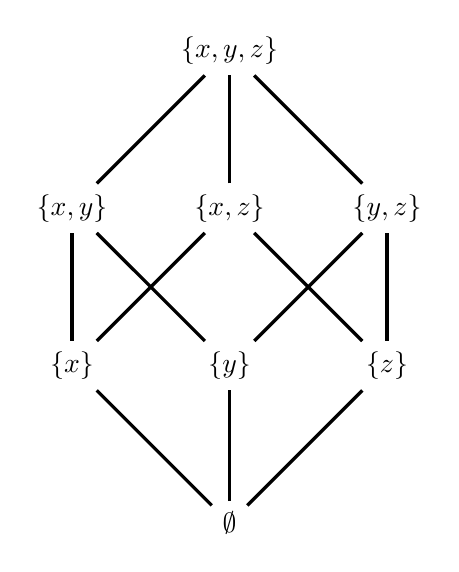
\begin{tikzpicture}[scale=2, very thick]
        % Nodes (subsets of {x, y, z})
        \node (xyz) at (0,2.5) {$\{x,y,z\}$};
        \node (xy) at (-1,1.5) {$\{x,y\}$};
        \node (xz) at (0,1.5) {$\{x,z\}$};
        \node (yz) at (1,1.5) {$\{y,z\}$};
        \node (x) at (-1,0.5) {$\{x\}$};
        \node (y) at (0,0.5) {$\{y\}$};
        \node (z) at (1,0.5) {$\{z\}$};
        \node (empty) at (0,-0.5) {$\emptyset$};

        % Edges (showing the subset relation)
        \draw (empty) -- (x);
        \draw (empty) -- (y);
        \draw (empty) -- (z);
        \draw (x) -- (xy);
        \draw (x) -- (xz);
        \draw (y) -- (xy);
        \draw (y) -- (yz);
        \draw (z) -- (xz);
        \draw (z) -- (yz);
        \draw (xy) -- (xyz);
        \draw (xz) -- (xyz);
        \draw (yz) -- (xyz);
    \end{tikzpicture}
    \caption{Hasse diagram of all subsets of the set $\{x,y,z\}$ with
    the subset relation.}
    \label{fig:hasse-diagram}
\end{figure}

\newpage

\begin{definition}{Total Order}{}
    Let $(A,\preceq)$ be a poset, if relation $\preceq$ satisfy that
    for any $x,y \in A$,
    \begin{equation*}
        x \preceq y \lor y \preceq x
    \end{equation*}
    then relation $\preceq$ is \textbf{totally order} on $A$ and we
    call that $A$ is a \textbf{toset}.
\end{definition}

\begin{remarks}
    sometimes we call that $x$ and $y$ are comparable if either $x
    \preceq y$ or $y \preceq x$.
\end{remarks}
\begin{definition}{Strict Order corresponding to $\preceq$}{}
    Let $(A,\preceq)$ be a poset, for any $x,y \in A$, we define
    \begin{equation*}
        x \prec y \iff  x \preceq y \land x \neq y
    \end{equation*}
    The relation $\prec$ on $A$ shall be called as the \textbf{strict
    order} corresponding to $\preceq$.
\end{definition}

\begin{remarks}
    strict order is obviously not partial order, because it is not
    reflexive. And $\succeq$ is just the inverse of $\preceq$. That is
    \begin{equation*}
        \succeq \ = \ \preceq^{-1}
    \end{equation*}
\end{remarks}

\begin{definition}{Maximal and Minimal}{}
    Let $(A,\preceq)$ be a poset,
    \begin{enumerate}

        \item a element $m \in A$ is called a \textbf{maximal} iff $m
            \nprec x \ \text{for all}\ x \in A$.
        \item a element $n \in A$ is called a \textbf{minimal} iff $x
            \nprec n \ \text{for all}\ x \in A$.

    \end{enumerate}

    That is to say there is no element in $A$ which is larger than $m$,
    and smaller than $n$.
\end{definition}

\begin{remarks}
    equivalently, the definitions can be reclaimed as
    \begin{enumerate}

        \item $\forall x \in A (m \preceq x \implies m = x)$
        \item $\forall x \in A (x \preceq n \implies x = n)$

    \end{enumerate}
\end{remarks}

\begin{examples}
    The Diagram below shows that minimal and maximal may not be
    unique in the set.
\end{examples}

\begin{figure}[ht]
    \centering
    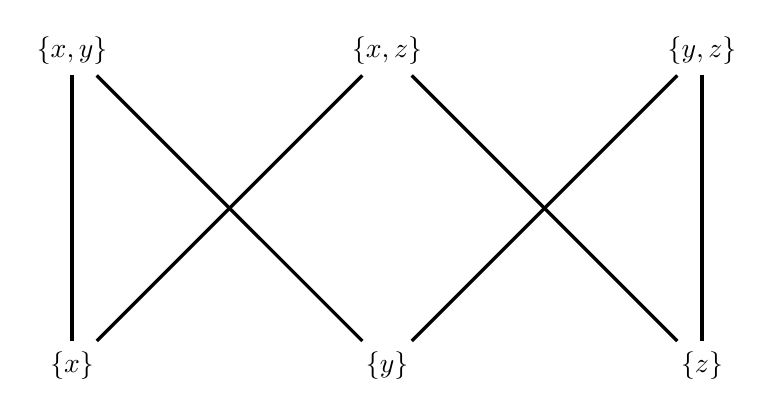
\begin{tikzpicture}[scale=2.0, very thick]
        % Define the nodes
        \node (xy) at (0,2) {$\{x, y\}$};
        \node (xz) at (2,2) {$\{x, z\}$};
        \node (yz) at (4,2) {$\{y, z\}$};

        \node (x) at (0,0) {$\{x\}$};
        \node (y) at (2,0) {$\{y\}$};
        \node (z) at (4,0) {$\{z\}$};

        % Draw the edges
        \draw (x) -- (xy);
        \draw (y) -- (xy);
        \draw (x) -- (xz);
        \draw (z) -- (xz);
        \draw (y) -- (yz);
        \draw (z) -- (yz);
    \end{tikzpicture}
    \caption{Hasse diagram of all subsets of \{x, y, z\} except the
    empty set and \{x, y, z\} itself.}
\end{figure}

\begin{definition}{Greatest and Least}{}
    Let $(A,\preceq)$ be a poset,
    \begin{enumerate}

        \item a element $m \in A$ is called a \textbf{greatest} iff $x
            \preceq m \ \text{for all}\ x \in A$.
        \item a element $n \in A$ is called a \textbf{least} iff $n
            \preceq x \ \text{for all}\ x \in A$.

    \end{enumerate}

\end{definition}

\begin{remarks}
    If the greatest and least exists, then they must be unique, the
    proof is trivial.
\end{remarks}

\begin{proposition}{}{}
    Let $(A,\preceq)$ be a poset, if the greatest $m$ exists, then $m$
    is also the maximal. In same way, if the least $n$ exists, then $n$
    is also the minimal.
\end{proposition}

\begin{proof}
    We just proof the first claim. Let $m$ be the greatest element.
    For any $x \in A$.
    \begin{align*}
        &m \preceq x\\
        &\implies m \preceq x \land x \preceq m\\
        &\implies m = x
    \end{align*}
\end{proof}

\begin{theorem}{}{}
    Let $(A,\preceq)$ be a toset. If the maximal exists, then it is
    also the greatest element and unique.
    If the minimal exists, then it is also the least element and unique.
\end{theorem}

\begin{proof}
    We proof the first claim. Let $m$ be the maximal. For any $x \in A$,
    \begin{align*}
        &m \preceq x \implies m = x\\
        &m \preceq x \lor x \preceq m \ \text{(definition of toset)}\\
        &\implies m = x \lor x \preceq m \ \text{and}\  m = x
        \implies x \preceq m\\
        &\implies x \preceq m
    \end{align*}
    The uniqueness is due to the uniqueness of the greatest element.
\end{proof}

\subsection{Functions}

\begin{definition}{Single-valued}{}
    A relation $R$ is \textbf{Single-valued} if for every $x \in dom
    R$, there is exactly one $y$ s.t. $\langle x,y \rangle \in R$. In
    other words
    \begin{equation*}
        \langle x,y \rangle \in R \land \langle x,z \rangle \in R \implies y = z
    \end{equation*}
\end{definition}

\begin{definition}{Functions}{}
    A \textbf{function} is a single-valued relation.
\end{definition}

\begin{definition}{Functions from A to B}{}
    Let $A$ and $B$ be sets, and $F$ be a relation from $A$ to $B$. Then $F$ is
    said to be a \textbf{function from $A$ to $B$} if following
    conditions holds:
    \begin{enumerate}

        \item $dom(F) = A$.
        \item $F$ is single-valued.

    \end{enumerate}
    The $A$ is \textbf{domain} of $F$, and $B$ is the
    \textbf{codomain} of $F$.\\
    We usually call that a function $F$ from $A$ to $B$ is a subset of
    $A \times B$ s.t. for each $x \in A$, there is exactly one $y \in
    B$ so that $\langle x,y \rangle \in F$.
\end{definition}

We write \underline{$F : A \to B$ to denote that $F$ is a function
from the set $A$ to the set $B$.} Thus, for each $x \in A$, there is
exactly one $y \in B$ such that $\langle x, y \rangle \in F$. This
unique $y$ is called \underline{“the value of $F$ at $x$” and is
denoted by $F(x)$.} Therefore, $\langle x, y \rangle \in F$ if and
only if $F(x) = y$.
Moreover, one can also say that \underline{the function $F$ maps $x$
to $F(x)$, denoted by $x \mapsto F(x)$.}

\begin{examples}
    Arrow diagram with domain as a red ellipse and codomain as a green
    ellipse representing the function \( F: A \to B \) defined by \( F
        = \{\langle a, 3 \rangle, \langle b, 5 \rangle, \langle c, 1
    \rangle, \langle d, 3 \rangle\} \)
\end{examples}

\begin{figure}[htbp]
    \centering
    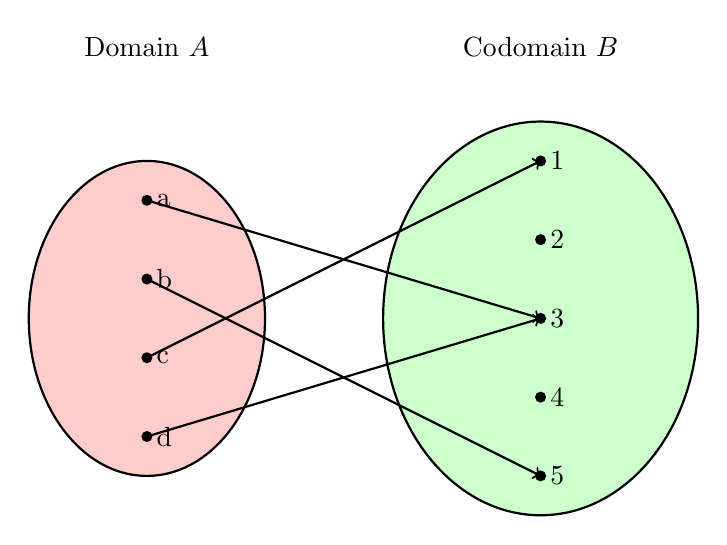
\begin{tikzpicture}

        % Red ellipse for domain A and green ellipse for codomain B
        \draw[thick, fill=red!20] (-2, 2.5) ellipse [x radius=1.5, y
        radius=2] node[above=3.2cm] {Domain \( A \)};
        \draw[thick, fill=green!20] (3, 2.5) ellipse [x radius=2, y
        radius=2.5] node[above=3.2cm] {Codomain \( B \)};

        % Black dots for elements of A inside the red ellipse
        \fill[black] (-2,4) circle (2pt) node[right] {a};
        \fill[black] (-2,3) circle (2pt) node[right] {b};
        \fill[black] (-2,2) circle (2pt) node[right] {c};
        \fill[black] (-2,1) circle (2pt) node[right] {d};

        % Black dots for elements of B inside the green ellipse
        \fill[black] (3,4.5) circle (2pt) node[right] {1};
        \fill[black] (3,3.5) circle (2pt) node[right] {2};
        \fill[black] (3,2.5) circle (2pt) node[right] {3};
        \fill[black] (3,1.5) circle (2pt) node[right] {4};
        \fill[black] (3,0.5) circle (2pt) node[right] {5};

        % Thicker arrows representing the function
        \draw[thick,->] (-2,4) -- (3,2.5); % a -> 3
        \draw[thick,->] (-2,3) -- (3,0.5); % b -> 5
        \draw[thick,->] (-2,2) -- (3,4.5); % c -> 1
        \draw[thick,->] (-2,1) -- (3,2.5); % d -> 3

    \end{tikzpicture}
    \caption{Arrow diagram representing the function \( F: A \to B \)
        defined by \( F = \{\langle a, 3 \rangle, \langle b, 5 \rangle,
    \langle c, 1 \rangle, \langle d, 3 \rangle\} \)}
    \label{fig:arrow-diagram}
\end{figure}

\begin{example}
    $F(x) = 2x^3 + 1,\ \text{for all } x \in \mathbb{R}.$ is a
    function, we can rewrite it in formal way:
    \begin{equation*}
        F = \{\langle x,y \rangle \in \mathbb{R}\times \mathbb{R}: y
        = 2 x^{3} + 1\}
    \end{equation*}
\end{example}

\begin{figure}[h]
    \centering
    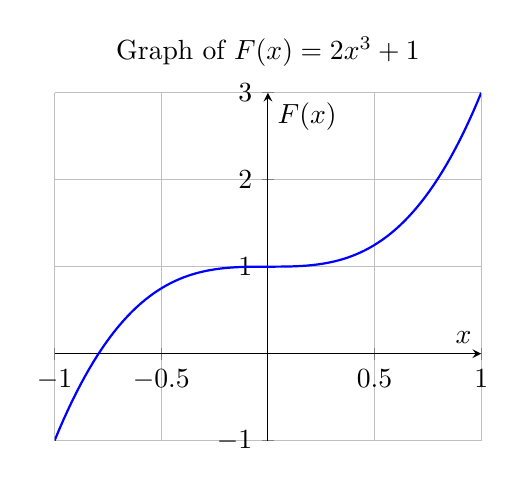
\begin{tikzpicture}
        \begin{axis}[
                axis lines = middle,
                xlabel = \( x \),
                ylabel = \( F(x) \),
                domain = -1:1,
                samples = 100,
                grid = both,
                title = {Graph of \( F(x) = 2x^3 + 1 \)},
                width = 7cm,
                height = 6cm
            ]
            \addplot[
                blue,
                thick
            ]
            {2*x^3 + 1};
        \end{axis}
    \end{tikzpicture}
    \caption{Graph of the function \( F(x) = 2x^3 + 1 \) for all \( x
    \in \mathbb{R} \)}
    \label{fig:graph}
\end{figure}

\begin{theorem}{}{}
    Let $F$ and $G$ be functions with common domain s.t. $domF = domG$. Then
    \[
        F = G \iff F(x) = F(y) \ \text{for all}\ x, y \in domF.
    \]
\end{theorem}

\begin{definition}{}{}
    Let $A$ and $B$ be sets. The set of all functions from $A$ to $B$,
    denoted by $B^A$, is defined by
    \[
        B^A = \{ F : F : A \to B \}.
    \]
\end{definition}

\begin{remarks}
    The existence of $B^{A}$ is guaranteed by \Cref{class} due to that
    $F \in \mathcal{P}(A \times B) $.
\end{remarks}

\begin{examples}
    The empty function is the function whose domain is empty set. For
    every set $B$, there is a unique empty function $f: \varnothing \to
    B$. Due to $f \subseteq \varnothing \times B$, which is just empty
    set,  the empty function is just empty set.
    \[
        B^{\varnothing} = \{\varnothing\}
    \]
    and
    \[
        \varnothing^A = \varnothing
    \]
\end{examples}

\begin{definition}{Operations on Functions}{}
    Let $F$ and $G$ be functions, and given set $A$
    \begin{enumerate}

        \item the \textbf{inverse} of $F$ is the \underline{relation}
            \begin{equation*}
                F^{-1} = \{\langle y,x \rangle : F(x) = y\}
            \end{equation*}
            or
            \begin{equation*}
                \langle y,x \rangle \in F^{-1} \iff F(x) = y
            \end{equation*}
        \item the \textbf{restriction} of $F$ to $A$ is the function
            \begin{equation*}
                F \vert_{A} = \{\langle x,y \rangle : F(x) = y \land x \in A\}
            \end{equation*}
        \item the \textbf{image} of $A$ under $F$ is the set
            \begin{equation*}
                F[A] = \{y : \exists x \in A (F(x) = y)\} = \{F(x): x \in A\}
            \end{equation*}
        \item the \textbf{inverse image} of $B$ under $F$ is the set
            \begin{equation*}
                F^{-1}[B] = \{x : \exists y \in B(F(x) = y)\} = \{x :
                F(x) \in B\}
            \end{equation*}
        \item the \textbf{composition} of $F$ and $G$ is the function
            \begin{equation*}
                F \circ G = \{\langle x,z \rangle : \exists y (G(x)=y
                \land F(y)=z)\}
            \end{equation*}
    \end{enumerate}
\end{definition}

\subsubsection{One-to-one Functions}
If a function has no repeated values, then we will say that the
function is one-to-one.
For example:

\begin{figure}[h]
    \centering
    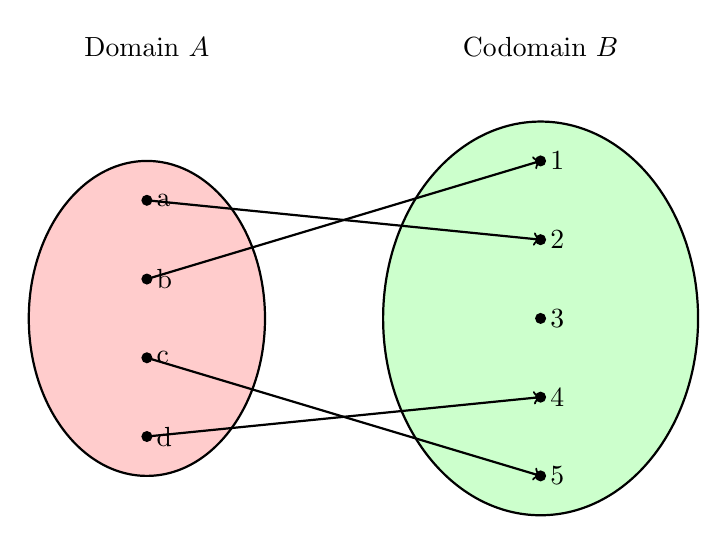
\begin{tikzpicture}

        % Red ellipse for domain A and green ellipse for codomain B
        \draw[thick, fill=red!20] (-2, 2.5) ellipse [x radius=1.5, y
        radius=2] node[above=3.2cm] {Domain \( A \)};
        \draw[thick, fill=green!20] (3, 2.5) ellipse [x radius=2, y
        radius=2.5] node[above=3.2cm] {Codomain \( B \)};

        % Black dots for elements of A inside the red ellipse
        \fill[black] (-2,4) circle (2pt) node[right] {a};
        \fill[black] (-2,3) circle (2pt) node[right] {b};
        \fill[black] (-2,2) circle (2pt) node[right] {c};
        \fill[black] (-2,1) circle (2pt) node[right] {d};

        % Black dots for elements of B inside the green ellipse
        \fill[black] (3,4.5) circle (2pt) node[right] {1};
        \fill[black] (3,3.5) circle (2pt) node[right] {2};
        \fill[black] (3,2.5) circle (2pt) node[right] {3};
        \fill[black] (3,1.5) circle (2pt) node[right] {4};
        \fill[black] (3,0.5) circle (2pt) node[right] {5};

        % Thicker arrows representing the function
        \draw[thick,->] (-2,4) -- (3,3.5); % a -> 2
        \draw[thick,->] (-2,3) -- (3,4.5); % b -> 1
        \draw[thick,->] (-2,2) -- (3,0.5); % c -> 5
        \draw[thick,->] (-2,1) -- (3,1.5); % d -> 4

    \end{tikzpicture}
    \caption{Arrow diagram representing the function \( F: A \to B \)
        defined by \( F = \{\langle a, 2 \rangle, \langle b, 1 \rangle,
    \langle c, 5 \rangle, \langle d, 4 \rangle\} \)}
    \label{fig:injection}
\end{figure}

\begin{definition}{Injection}{}
    A function $F$ is said to be \textbf{one-to-one}, or
    \textbf{injection} iff for any $x, y \in domF$
    \begin{equation*}
        F(x) = F(y) \implies x = y
    \end{equation*}
    In other words, distinct elements are mapped to distinct elements.
\end{definition}

\begin{lemma}{}{}
    A function $F$ is one-one iff it is single-rooted.
\end{lemma}

\begin{theorem}{}{}
    Let $F$ be a relation.
    \begin{enumerate}

        \item Then $F^{-1}$ is a function iff $F$ is single-rooted.
        \item Then $F$ is a function iff $F^{-1}$ is single-rooted.

    \end{enumerate}
\end{theorem}

\begin{proof}
    ($\implies $)\\
    To proof $F$ is single-rooted, Suppose
    \begin{align*}
        &\langle x,z \rangle \in F \land \langle y,z \rangle \in F\\
        &\implies \langle z,x \rangle \in F^{-1} \land \langle z,y
        \rangle \in F^{-1} \\
        &\implies x = y
    \end{align*}

    ($\Leftarrow $)
    To proof $F^{-1}$ is single-valued, Suppose
    \begin{align*}
        &\langle z,x\rangle \in F^{-1} \land \langle z,y \rangle \in F^{-1}\\
        &\implies \langle x,z \rangle \in F \land \langle y,z \rangle \in F\\
        &\implies x = y
    \end{align*}
\end{proof}

\begin{corollary}{}{}
    $F$ is a one-one function, $F^{-1}$ is also a one-one function.
\end{corollary}

\begin{proof}
    Firstly, $F$ is single-rooted implies $F^{-1}$ is a function. Then
    $F$ is a function implies $F^{-1}$ is single-rooted. So $F^{-1}$ is one-one.
\end{proof}

\begin{theorem}{}{}
    Let $F$ be a one-one function.
    \begin{enumerate}

        \item $(F^{-1} \circ F)(x) = x$ for all $x \in domF$
        \item $(F \circ F^{-1})(y) = y$ for all $y \in ranF$

    \end{enumerate}
\end{theorem}

\begin{proof}
    for every $x \in domF$, there exits $y \in ranF$ s.t. $F(x) = y$.
    \begin{equation*}
        F^{-1} \circ F(x) = F^{-1}(F(x))
    \end{equation*}
\end{proof}

\begin{definition}{Surjection}{}
    A function $F : A \to B$ maps A \textbf{onto} B, or
    \textbf{surjection} iff $ranF = B$, that is for any $y \in B$
    \begin{equation*}
        \exists x \in A(F(x) = y)
    \end{equation*}
\end{definition}

\begin{figure}[h]
    \centering
    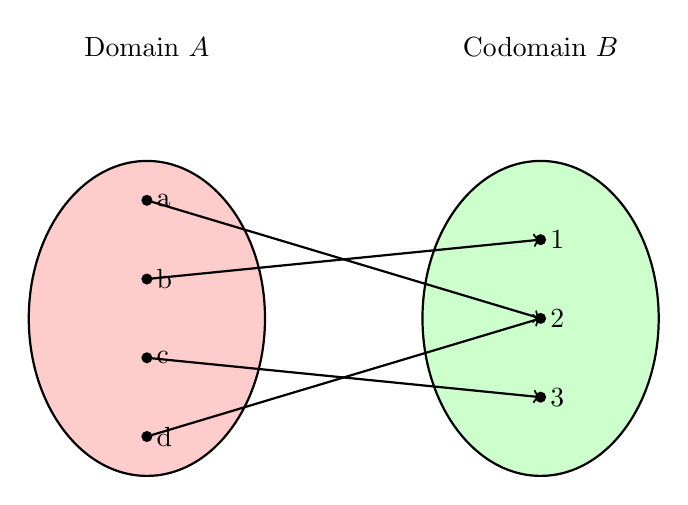
\begin{tikzpicture}

        % Red ellipse for domain A and green ellipse for codomain B
        \draw[thick, fill=red!20] (-2, 2.5) ellipse [x radius=1.5, y
        radius=2] node[above=3.2cm] {Domain \( A \)};
        \draw[thick, fill=green!20] (3, 2.5) ellipse [x radius=1.5, y
        radius=2] node[above=3.2cm] {Codomain \( B \)};

        % Black dots for elements of A inside the red ellipse
        \fill[black] (-2,4) circle (2pt) node[right] {a};
        \fill[black] (-2,3) circle (2pt) node[right] {b};
        \fill[black] (-2,2) circle (2pt) node[right] {c};
        \fill[black] (-2,1) circle (2pt) node[right] {d};

        % Black dots for elements of B inside the green ellipse
        \fill[black] (3,3.5) circle (2pt) node[right] {1};
        \fill[black] (3,2.5) circle (2pt) node[right] {2};
        \fill[black] (3,1.5) circle (2pt) node[right] {3};

        % Thicker arrows representing the function
        \draw[thick,->] (-2,4) -- (3,2.5); % a -> 2
        \draw[thick,->] (-2,3) -- (3,3.5); % b -> 1
        \draw[thick,->] (-2,2) -- (3,1.5); % c -> 3
        \draw[thick,->] (-2,1) -- (3,2.5); % d -> 2

    \end{tikzpicture}
    \caption{Arrow diagram representing the function \( F: A \to B \)
        defined by \( F = \{\langle a, 2 \rangle, \langle b, 1 \rangle,
    \langle c, 3 \rangle, \langle d, 2 \rangle\} \)}
    \label{fig:surjection}
\end{figure}

\begin{definition}{Bijection}{}
    A function $F : A \to B$ is injective and surjective is called a
    \textbf{bijection}. In other words, $F$ is one-one and onto $B$.
\end{definition}

\begin{theorem}{}{}
    If $F : A \to B$ is a bijection, then $F^{-1} : B \to A$ is also a
    bijection and
    \begin{enumerate}

        \item $(F \circ F^{-1})(x) = x$ for all $x \in A$
        \item $(F^{-1} \circ F)(y) = y$ for all $y \in B$

    \end{enumerate}

\end{theorem}

\subsubsection{Index Sets}

It is useful to identify the function $F$ by using the indexed
notation $\langle F_i : i \in I \rangle$ where $I$ is referred to as
the \underline{index set}, an element $i$ in $I$ is called an
\underline{index}, and each value $F_i$ of the function at an index
$i$ is called a \underline{term}. Thus, $\langle F_i : i \in I
\rangle$ will be said to have nonempty terms when $F_i \neq
\varnothing$ for all $i \in I$. We shall say that $\langle F_i : i
\in I \rangle$ is an \underline{indexed function}, and its range $\{
F_i : i \in I \}$ shall be called an \underline{indexed set}.

\begin{definition}{}{}
    Let $\{ F_i : i \in I \}$ be an indexed set. Define
    \[
        \bigcup_{i \in I} F_i = \bigcup \{F_{i} : i \in I\}
    \]
    that is,
    \[
        \bigcup_{i \in I}F_{i} = \{ x : x \in F_i \text{ for some } i \in I \}.
    \]
\end{definition}

\begin{definition}{}{}
    Let $\{ F_i : i \in I \}$ be an indexed set. Define
    \[
        \bigcap_{i \in I} F_i = \bigcap \{F_{i} : i \in I\}
    \]
    that is,
    \[
        \bigcap_{i \in I}F_{i} = \{ x : x \in F_i \text{ for all } i \in I \}.
    \]
\end{definition}

\newpage
\section{Natural Numbers}

\subsection{Peano Postulates}

\begin{definition}{}{}
  Let $S : N \to N$ and let $A \subseteq N$. Then $A$ is said to be
  closed under $S$ iff
  \begin{equation*}
    S(x) \in A \text{ for all } x \in A
  \end{equation*}
\end{definition}

\begin{definition}{Peano System}{}
  Let $(N,S,e)$ be an ordered triple that consists of a set $N$, a
  function $S : N \to N$, and an element $e \in N$. Then $(N,S,e)$
  is a \textbf{Peano system} if the following conditions hold:
  \begin{enumerate}

    \item $e \notin ranS$
    \item $S$ is injective.
    \item For all $A \subseteq N$
      \begin{equation*}
        e \in A \land A \text{ is closed under } S \implies A = N
      \end{equation*}

  \end{enumerate}

\end{definition}

\subsection{Natural Number Set $\omega$}

\subsubsection{Inductive Sets}

In this section, we will construct natural numbers under the
architecture of set theory.

\begin{definition}{Successor}{}
  For each set $x$, the \textbf{successor} $x^{+}$ is the set defined by
  \begin{equation*}
    x^{+} = x \cup \{x\}
  \end{equation*}
\end{definition}

\begin{proposition}{}{}
  \begin{enumerate}

    \item $a \in x^{+} \iff a \in x \lor a = x$
    \item $x \in x^{+}$
    \item $x \subseteq x^{+}$

  \end{enumerate}
\end{proposition}

\begin{example}
  The first few natural numbers as follows
  \begin{itemize}

    \item $0 = \varnothing$
    \item $1 = \{0\}$
    \item $2 = \{0,1\}$
    \item $3 = \{0,1,2\}$
    \item $4 = \{0,1,2,3\}$

  \end{itemize}
\end{example}

\begin{definition}{Inductive}{}
  A set $I$ is said to be \textbf{inductive} iff
  \begin{enumerate}

    \item $\varnothing \in I$
    \item $\forall a \in I (a^{+} \in I)$

  \end{enumerate}
  The second one can be also restated as "The set is closed under successor."
\end{definition}

\begin{lemma}{Infinity Axiom}{}
  There is a inductive set.
  \begin{equation*}
    \exists I (\varnothing \in I \land \forall x \in I(x^{+} \in I))
  \end{equation*}
\end{lemma}

\begin{definition}{Natural Numbers}{}
  A \textbf{natural number} is an element that belongs to every
  inductive sets. In other words, $x$ is a natural number iff
  $x$ in every inductive sets.
\end{definition}

\begin{definition}{Natural Number Set}{}
  There exits a unique set $\omega$ such that for all $x$
  \begin{equation*}
    x \in \omega \iff x \text{ in every inductive set}
  \end{equation*}
  We denote the set as
  \begin{equation*}
    \omega = \{x : x \text{ in every inductive set}\}
  \end{equation*}
\end{definition}

\begin{proof}
  By infinity axiom, there exits an inductive set $A$. And
  \begin{equation*}
    x \text{ in every inductive set } \implies x \in A.
  \end{equation*}
  By \Cref{class}, there is a unique set $\omega$ s.t.
  \begin{equation*}
    x \in \omega \iff x \text{ in every inductive set}
  \end{equation*}
\end{proof}

\begin{theorem}{}{}
  The set $\omega$ is inductive and is a subset of every inductive
  set. Hence $\omega$ is the \textbf{smallest inductive set}.
\end{theorem}

\begin{corollary}{Principle of Mathematical Induction}{label:PMI}
  If $I$ is inductive and $I \subseteq \omega$, then $I = \omega$.
\end{corollary}

\begin{remarks}
  Suppose $P(n)$ is some property. To prove by induction that
  \begin{equation*}
    \forall n \in \omega P(n)
  \end{equation*}
  We just let $I = \{n \in \omega : P(n)\} \subseteq \omega$
  If we can prove that
  \begin{enumerate}

    \item $0 \in I$
    \item $n \in I \implies n^{+} \in I$

  \end{enumerate}
  Then $I = \omega$, by \Cref{label:PMI}. Therefore $P(n)$ holds
  for all natural numbers.
\end{remarks}

\begin{theorem}{}{}
  For every $n \in \omega$, either $n = 0$, or $n = k^{+}$ for
  some $k \in \omega$.
\end{theorem}

\begin{proof}
  Let $I = \{n \in \omega: n = 0 \lor \exists k \in \omega(n = k^{+})\}$\\
  \begin{itemize}

    \item Obviously, $0 \in I$.
    \item Let $n \in I$, then $n = 0 \lor n = k^{+} \text{ for some }
      k \in \omega$.
      \begin{enumerate}

        \item If $n = 0$, then $n^{+} = 0^{+}$, so $n^{+} \in I$.
        \item If $n = k^{+} \ \text{for some}\ k \in \omega$, then $n^{+} =
          (k^{+})^{+}$, so $n^{+} \in I$.

      \end{enumerate}

  \end{itemize}
  By \Cref{label:PMI}, $I = \omega$.
\end{proof}

\subsubsection{Transitive Sets}

There are some other important properties on natural numbers, such as

\begin{enumerate}

  \item $0 \in 1 \in 2 \in 3 \in 4 \in ...$
  \item $0 \subseteq 1 \subseteq 2 \subseteq 3 \subseteq 4 \subseteq ...$

\end{enumerate}

\begin{definition}{Transitive Sets}{}
  The set $A$ is called a \textbf{transitive set} if $\forall x \in
  A(x \subseteq A)$. In other words, every member of $A$ is also a
  subset of $A$.\\
  or more rigorously
  \begin{equation*}
    A \text{ is transitive } \iff (\forall a \in A)(\forall x \in a)(x \in A)
  \end{equation*}
\end{definition}

\begin{proposition}{}{}
  Let $A$ be a set
  \begin{equation*}
    A \text{ is transitive } \iff \bigcup A \subseteq A
  \end{equation*}
\end{proposition}

\begin{proposition}{}{}
  Let $A$ be a transitive set. Then
  \begin{equation*}
    \bigcup A^{+} = A
  \end{equation*}
\end{proposition}

\begin{proof}

\end{proof}

\begin{proposition}{}{}
  For all $m,n \in \omega$, if $n^{+} = m^{+}$, then $n = m$.
\end{proposition}

\begin{theorem}{}{}
  Every natural number is transitive set.
\end{theorem}

\begin{proof}
  We proof by induction. Let
  \begin{equation*}
    I = \{ n \in \omega : n \text{ is transitive}\}
  \end{equation*}
  Clearly, $0 \in I$. Let $n \in I$. We need to show that $n^{+} \in
  I$ and just $\bigcup n^{+} \subseteq n^{+}$.\\
  Firstly, $\bigcup n^{+} = n$, and $n \subseteq n^{+}$, Hence
  \begin{equation*}
    \bigcup n^{+} \subseteq n^{+}
  \end{equation*}
  By induction, $I = \omega$.
\end{proof}

\begin{theorem}{}{}
  The set $\omega$ is a transitive set.
\end{theorem}

\begin{proof}
  we shall prove $\forall n \in \omega(n \subseteq \omega)$ by induction.
\end{proof}

\subsection{Recursion Theorem on $\omega$}

\newpage
\section{Size of Sets}

\subsection{Finite Sets}

\begin{definition}{Finite Set}{}
    A set $X$ is \textbf{finite} iff there exits an injection $f: X \to n$ for some natural number n.
\end{definition}

\begin{definition}{Number of elements}{}
    Suppose that $X$ is a finite set. Let $n$ be the least number s.t. there is 
    an injection $f: X \to n$. Then $n$ is the \textbf{number of elements} in $X$, 
    and we write $|X| = n$.
\end{definition}

\begin{theorem}{}{}
    Let $A$ be finite and $|A| = n$. If $f: A \to n$ is injective, then $f$ is surjective.
\end{theorem}

\begin{proof}
    If $A$ is empty, then $f$ is vacuously surjective. Assume $A$ is not empty. 
    Suppose $f$ is not surjective, and let $k \in n \text{\ and\ } k \notin ran(f)$. 
\end{proof}

\begin{corollary}{}{}
    If $A$ is finite and $|A| = n$, then there is a bijection $f: A \to n$.
\end{corollary}

\begin{theorem}{}{}
    Let $f: A \to A$ be injective and $A$ is finite. Then $f$ is surjective.
\end{theorem}

\begin{corollary}{Property of infinite set}{}
    Let $f: A \to A$ be injective and not surjective. Then $A$ is infinite.
\end{corollary}

\begin{theorem}{}{}
    Let $A$ and $B$ be finite sets. Then there is a bijection $f: A \to B$ iff $|A| = |B|$.
\end{theorem}

\begin{theorem}{}{}
    For all natural numbers $n$, $|n| = n$.
\end{theorem}

\begin{proof}{}{}
    
\end{proof}

\begin{corollary}{Pigeonhole Principle}{}
    Let $m$ and $n$ be natural numbers and $f: n \to m$. If $m < n$, then $f$ is not injective.
\end{corollary}

\begin{theorem}{}{}
    The set $\omega$ is an infinite set.
\end{theorem}

\begin{corollary}{}{}
    If $G: \omega \to A$ is injective, then $A$ is an infinite set.
\end{corollary}

\begin{lemma}{Dual version of Pigeonhole Principle}{}
    If $m < n$ and $f: m \to n$, then $f$ is not surjective.
\end{lemma}

\begin{theorem}{}{}
    If $N$ is finite and $f: N \to N$ is surjective, then $f$ is injective.
\end{theorem}

\begin{theorem}{}{}
    If $A$ is a finite set, then $\mathcal{P}(A)$ is finite.
\end{theorem}

\subsection{Countable Sets}

\begin{definition}{Countable Set}{}
    A set $X$ is countable iff there is injection $f :X \to \omega$.
\end{definition}

\begin{definition}{}{}
    A set $X$ is countably infinite iff it is countable and infinite.
\end{definition}

\begin{theorem}{}{}
    Let $A$ and $B$ are sets where $B$ is countable. If there is an
    injection $f: A \to B$, then $A$ is countable.
\end{theorem}

\begin{theorem}{}{}
    If $B$ is countable set and $A \subset B$, then $A$ is countable.
\end{theorem}

\newpage

\end{document}
